\documentclass{report}
\usepackage[english]{babel}
\usepackage[utf8]{inputenc}
\usepackage[T1]{fontenc}
\usepackage[hidelinks]{hyperref}
\usepackage[fixlanguage]{babelbib}
\usepackage{pgfplots}
\pgfplotsset{width=7cm,compat=1.18}
\usepackage{float}
\usepackage{subcaption}
\usepackage{booktabs}
\usepackage{amsmath}
\usepackage{array}
\usepackage{amssymb}
\usepackage{systeme}
\usepackage{tikz}
\usepackage{verbatim}
\usepackage{listings}
\usepackage{lipsum}
\usepackage{cite}

\begin{document}

\pagenumbering{gobble}

\begin{titlepage}
    \begin{figure}[!htb]
        \centering
        
\includegraphics[keepaspectratio=true,scale=0.5]{cherubinFrontespizio.eps}
    \end{figure}
    
    \begin{center}
        \LARGE{UNIVERSITÀ DI PISA}
        \vspace{5mm}
        \\ \large{DEPARTMENT OF COMPUTER ENGINEERING}
    \end{center}
    
    \vspace{15mm}
    \begin{center}
        {\LARGE{\bf Edge Computing\\Project Documentation}}
    \end{center}
    \begin{center}
        {
        \makeatletter    
        \@date
        \makeatother    
        }
    \end{center}
    \vspace{30mm}
    
    \begin{minipage}[t]{0.47\textwidth}
        {\large{Team:}{\normalsize\vspace{3mm} \bf\\ \large{Cavedoni F.\\Monaci M.\\Pinna F.}}}
    \end{minipage}
    
    \vspace{15mm}
    \hrulefill
    \\\centering{\large{ACADEMIC YEAR 2024/2025}}
\end{titlepage}

\newpage
\tableofcontents
\newpage

\pagenumbering{arabic}
\setcounter{page}{1}

\chapter{Introduction}
A cellular network is composed of M base stations, placed within a 2D floorplan of size L $\times$ H
according to a regular grid. Each base station also has edge computing capabilities, i.e., it can receive
computing tasks from cellular network's users and serve them at a rate equal to S instructions per
seconds following a First Come First Served (FCFS) policy. Assume that all base stations are
interconnected between each other via mesh topology.
\section{Problem description}
We consider N users placed at random locations \texttt{(x, y)} within the same 2D floorplan, where coordinates
\texttt{x} and \texttt{y} are random variables to be defined later. Each user generates a new computing task request
every T seconds, and each request consists of I instructions to be executed. T and I are exponentially
distributed RVs. In particular, a user sends each new task request to its serving base station (i.e., the
closest one), which in turn can follow one of methods below:
\begin{itemize}
    \item [\textbf{a)}] serve the request locally
    \item [\textbf{b)}] forward the request to the less-loaded base station
\end{itemize}

\section{Objectives}
This project aims to fulfill the following:
\begin{itemize}
    \item Evaluate the time required to complete a computing task for various values of N comparing method a) against method b)
    \item Evaluate the following scenarios:
    
    \texttt{x} and \texttt{y} are \textit{uniform distributed} random variables in range \[x\in[0, width] \quad y\in[0, height]\]

    \texttt{x} and \texttt{y} are distributed as a \textit{lognormal distribution} with parameters defined in \autoref{factors}
    \item \texttt{TODO\dots}
\end{itemize}

\section{Performance indexes}
\begin{itemize}
    \item Response time of the system (when a packet leaves the system)
    \item Response time of each queue
    \item Packet loss
    \item \texttt{TODO\dots}
\end{itemize}

\chapter{Modeling}
Our system is described by the following scheme
\begin{figure}[H]
    \centering
    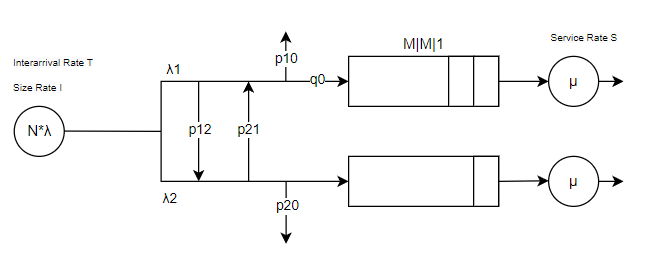
\includegraphics[width=\textwidth]{immagine.png}
    \caption{Scheme}
    \label{scheme}
\end{figure}

As shown in \autoref{scheme}, each base station is modeled as an \texttt{M/M/1/k} system, as rates $\lambda_i$ and $\mu_i$ are exponentially distributed random variables $\forall \ i \in [1, M]$.

\section{Assumptions}
We make some assumption in order to simplify the implementation of the system.

\begin{enumerate}
    \item Rerouting propagation delay is constant for each base station.
    \item Every job entering a queue is destined to be served and cannot exit the queue in any other way.
    \item Each queue length is \textit{finite} with \texttt{k} slots.
    \item \textit{(work in progress)} Width and height of the grid are such that it results in a square area.
\end{enumerate}

\section{Factors description}\label{factors}
\begin{itemize}
    \item \texttt{N}: number of users
    \item \texttt{k}: length of each queue
    \item $\lambda_i$: Interarrival rate for base station $i$
    \item $\mu$: Service rate for each base station
    \item $\mu_{log}$: Average of lognormal distribution
    \item $\sigma_{log}$: Standard deviation of lognormal distribution
\end{itemize}

\chapter{Implementation}
\section{Modules}
The following modules have been defined:
\begin{itemize}
    \item \textbf{EdgeNetwork}: compound module which represents the system and hosts the following simple modules
    \begin{itemize}
        \item \textbf{BaseStation}: simple module which receives, precesses and (in case of scenario b) forwards packets sent by users according to the specified distribution. 
        \item \textbf{User}: simple module which generates and sends packets (with length dependent by the specified distribution) to the nearest base station.
    \end{itemize}    
\end{itemize}

\section{Modules' behaviour}
\subsection{EdgeComputingNetwork}
\begin{itemize}
    \item Hosts base stations and users physically and memorizes their parameters in order to retreive them during the simulation via parent pointers.
\end{itemize}
\subsection{BaseStation}
\begin{itemize}
    \item Receives packets from users in form of \texttt{cMessage} objects and depending on the current scenario performs one of the following actions:
    \begin{itemize}
        \item [\textbf{Locally managed:}] if the queue has enough free slots the base station enqueues the packet to be processed, ignoring all other base stations.
        \item [\textbf{Forwarding:}] when a packet is received the base station searches for the base statio with the lowest load on their queue and forwards the packet to it. If and only if every other base station has a higher load, the packet is served locally.
    \end{itemize}
    \item It also records statistics every time a packet is \textit{dropped} or \textit{forwarded} (as number of packets) and about \textit{queue length} and \textit{response time} (in order to compute its average).
\end{itemize}

\subsection{User}
\begin{itemize}
    \item Generates packets with length and rate which are exponentially distributed and sends them to the \textit{nearest}\footnote{According to the euclidean distance}
    % non so se è superfluo specificarlo
    \texttt{BaseStation}.
\end{itemize}

\chapter{Verification}
Right away we describe the tests made to verify if our system tends to remain stable under extreme conditions or degenerate ones.

\section{Scenario 1 - no users}
As we expect in this degenerate case the system remains stable as there is nothing for it to precess or forward.

\section{Scenario 2 - very high number of users}
In this case we test our system against an enormous number of users and just a few base stations ($M=2 \ N=100$)

The system results to be robust to this kind of issue, maintaining a stable \textit{queue length} and a consistent \textit{response time}, as shown in \autoref{avg_ql_2} and \autoref{avg_rt_2}

\begin{figure}[H]
    \centering
    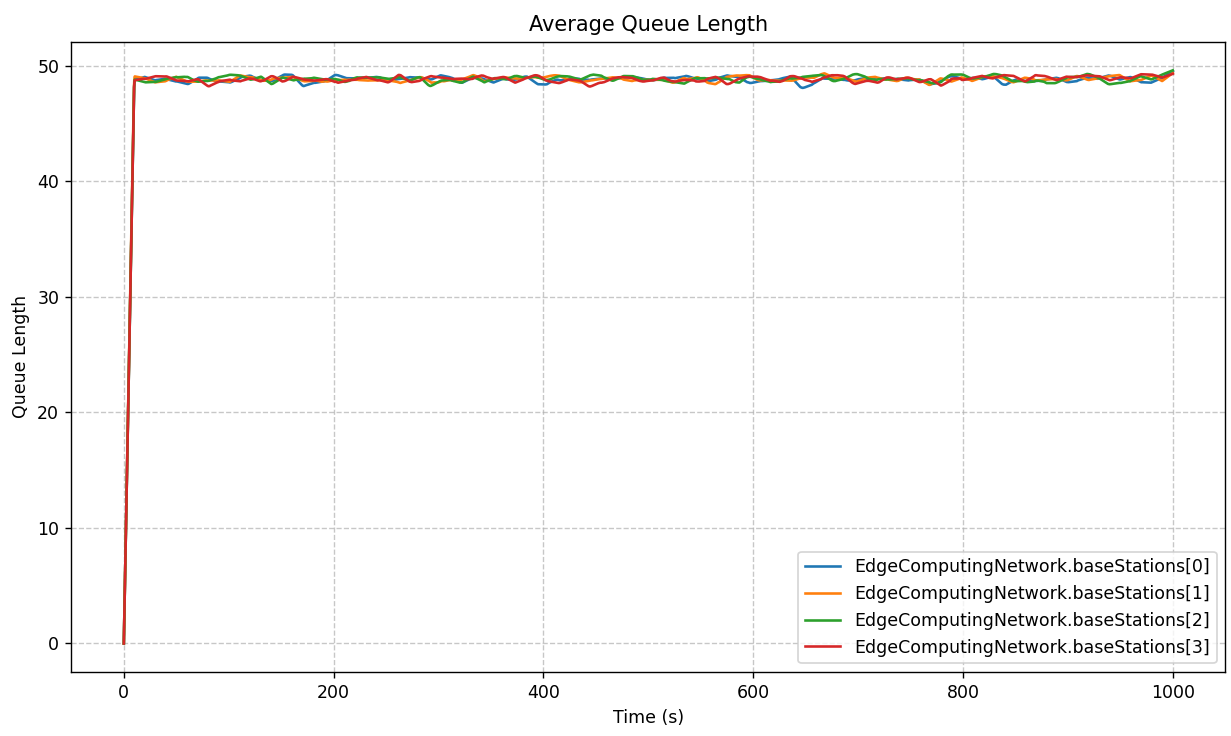
\includegraphics[width=0.8\textwidth]{avg_ql_2.png}
    \caption{}
    \label{avg_ql_2}
\end{figure}
\begin{figure}[H]
    \centering
    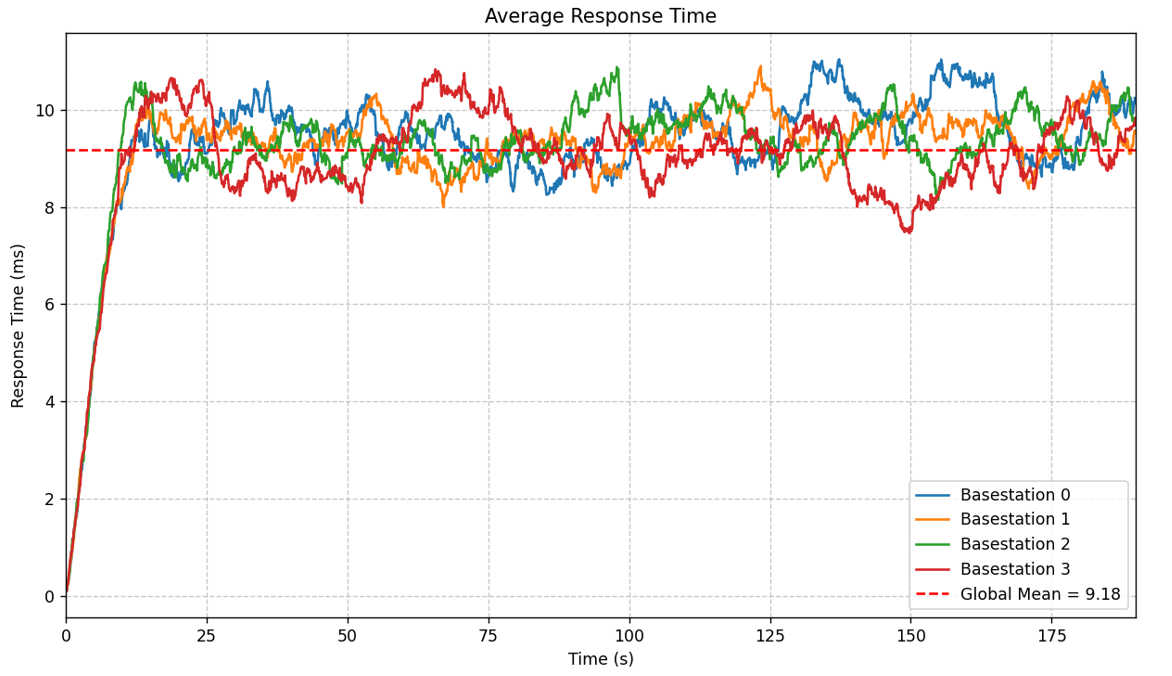
\includegraphics[width=0.8\textwidth]{avg_rt_2.png}
    \caption{}
    \label{avg_rt_2}
\end{figure}

\section{Scenario 3 - very small service rate}
Now we want to know how the system reacts when the service rate is a lot lower than the interarrival rate.

Throughout simulations we find that the queue length tends to be stable after about $50s$ (\autoref{avg_ql_3}). Instead the response time has a \textit{linear behaviour} over time (\autoref{avg_rt_3}).

\begin{figure}[H]
    \centering
    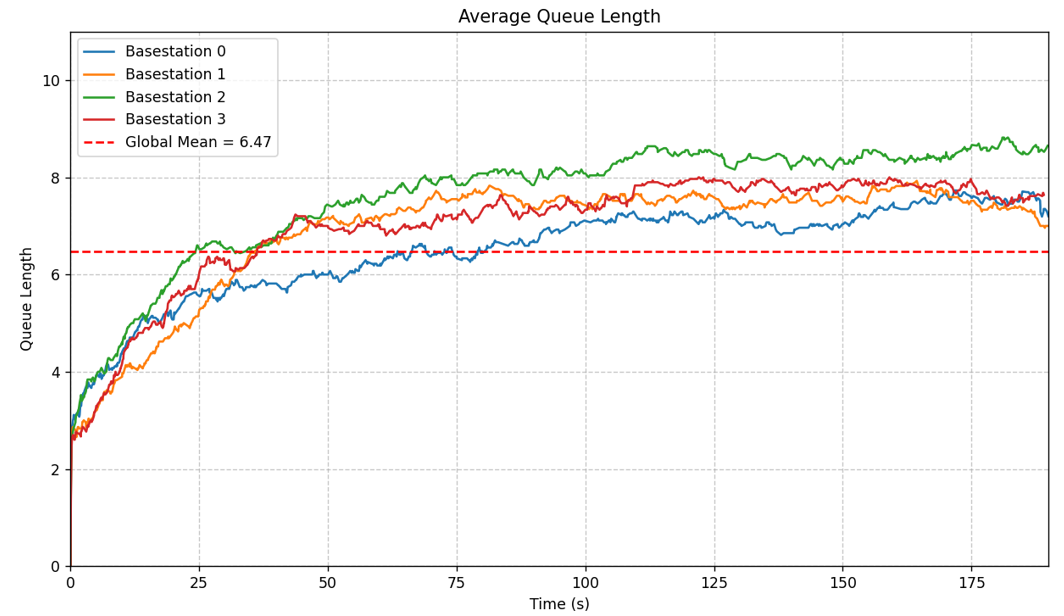
\includegraphics[width=0.8\textwidth]{avg_ql_3.png}
    \caption{}
    \label{avg_ql_3}
\end{figure}
\begin{figure}[H]
    \centering
    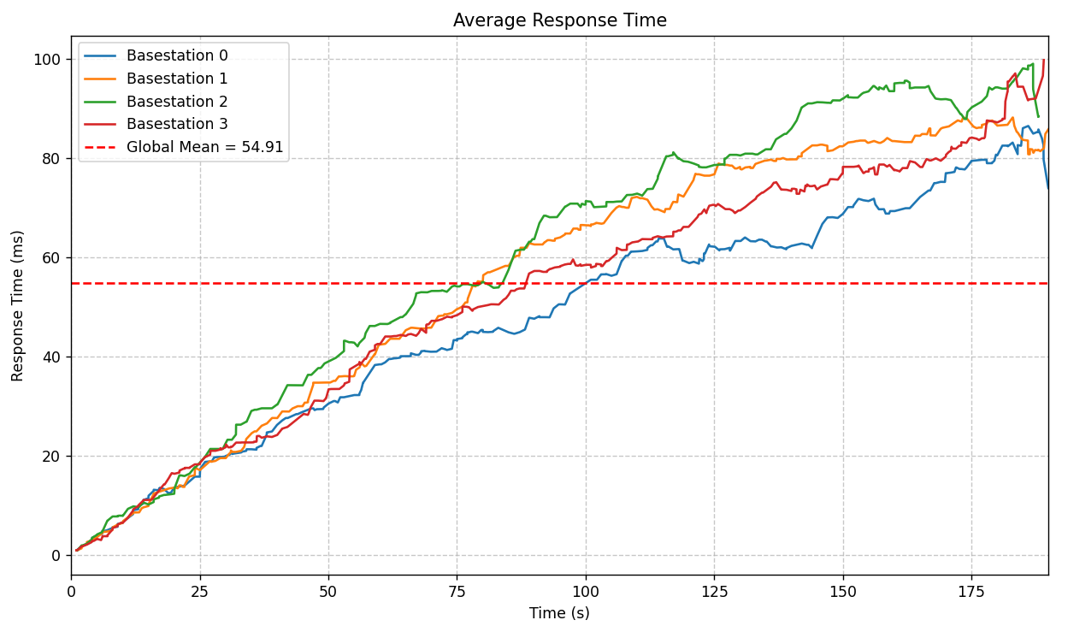
\includegraphics[width=0.8\textwidth]{avg_rt_3.png}
    \caption{}
    \label{avg_rt_3}
\end{figure}

\section{Consistency test}
In this test we verify that the system produces coherent results in both configurations and those results to be feasible.

We compare the results of simulations in both `\textit{Locally managed}' and `\textit{Forwarding}' configuration.

It is clear that in both cases we end up with similar means ($\Delta=1.22$), even though forwarding configuration is slightly better. What catches the eye is the difference between the variation of the two cases, once again favoring the forwarding.

\begin{figure}[H]
    \begin{subfigure}{0.60\textwidth}
        \centering
        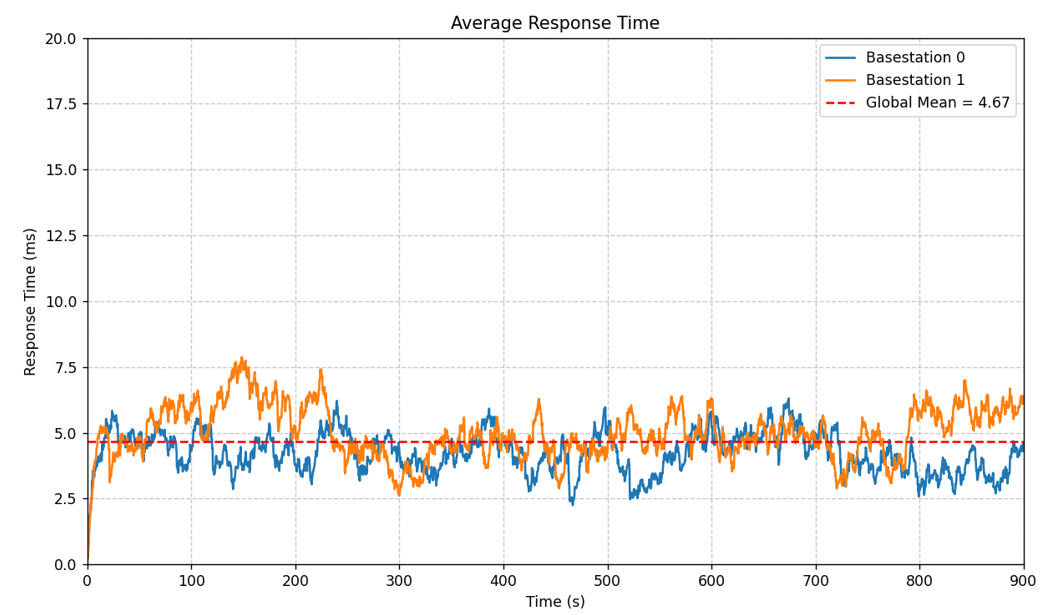
\includegraphics[width=0.8\textwidth]{avg_rt_a.png}
        \caption{Locally managed}
    \end{subfigure}
    \begin{subfigure}{0.60\textwidth}
        \centering
        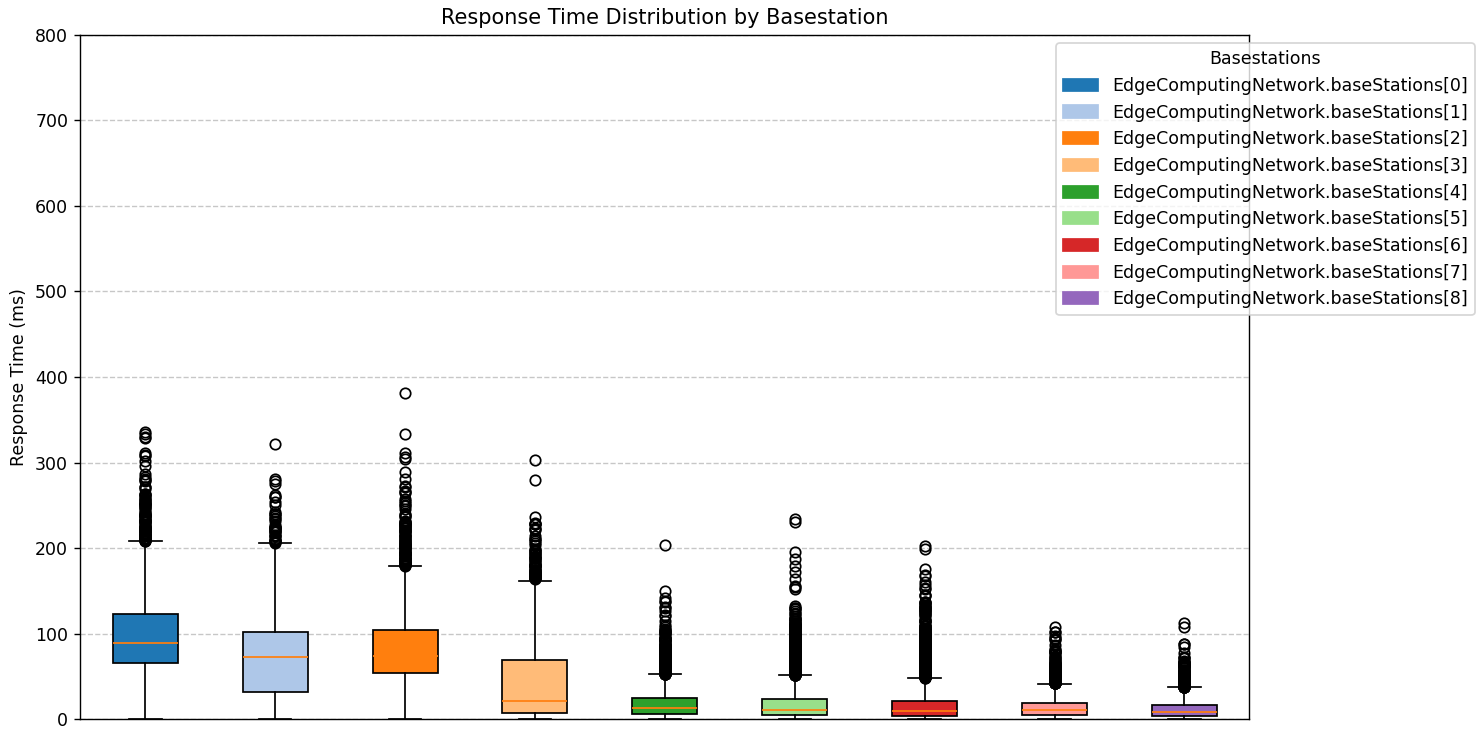
\includegraphics[width=0.8\textwidth]{avg_rt_b.png}
        \caption{Forwarding}
    \end{subfigure}
\end{figure}

\section{Continuity test}
This test ensures that the system responds without discontinuity while gradually varying the parameters.

We inspect the response time while incrementing two parameters: the number of users and the interarrival rate.

\subsection{Increment of users - ($10, \ 50, \ 100$)}\label{nusers}
As we might expect the response time becomes higher with the rising of the number of users but the mean always remains under $10s$. Once the system is underway, it remains stable with the majority of the oscillations belonging to the case $N=50$ (\autoref{rt_50})

\begin{figure}[H]
    \begin{subfigure}{0.55\textwidth}
        \centering
        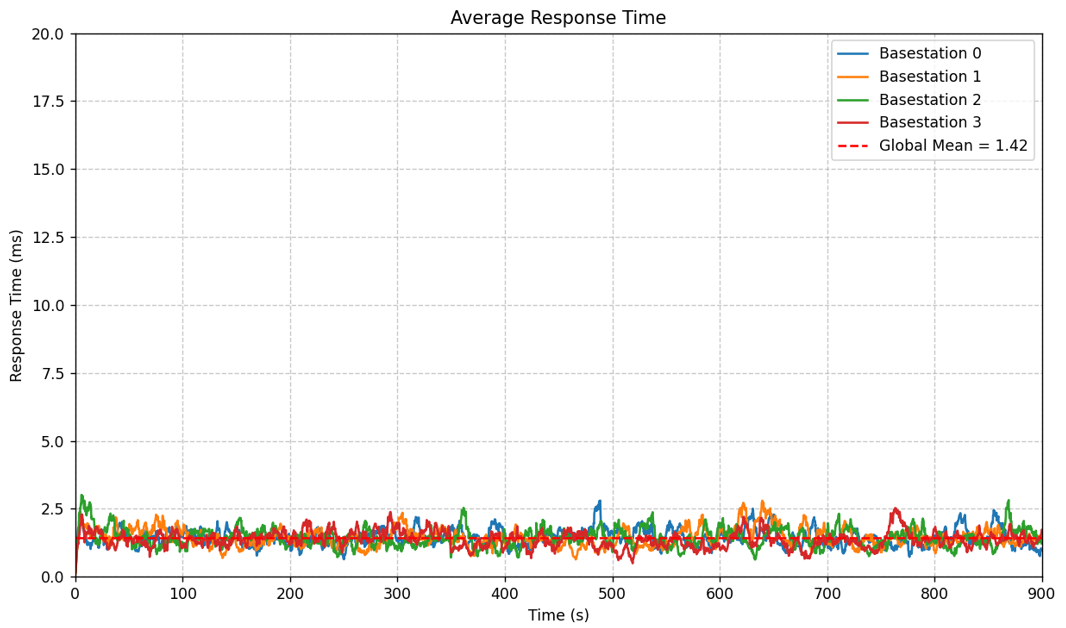
\includegraphics[width=0.8\textwidth]{rt_10.png}
        \caption{$N=10$}
    \end{subfigure}
    \begin{subfigure}{0.55\textwidth}
        \centering
        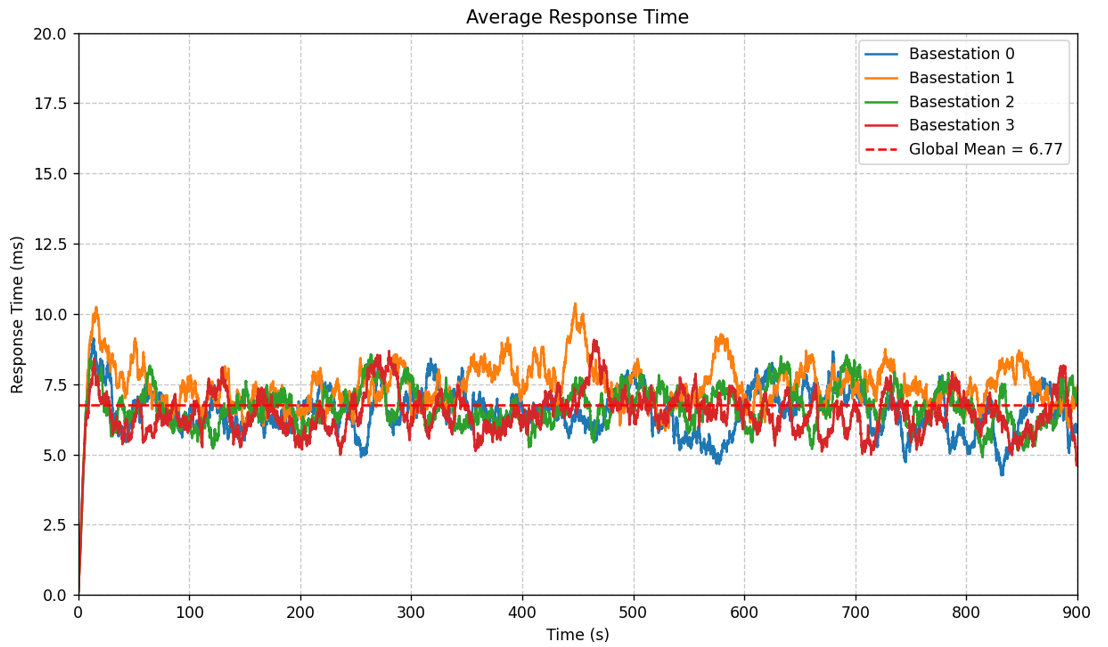
\includegraphics[width=0.8\textwidth]{rt_50.png}
        \caption{$N=50$}
        \label{rt_50}
    \end{subfigure}
    \begin{subfigure}{0.55\textwidth}
        \centering
        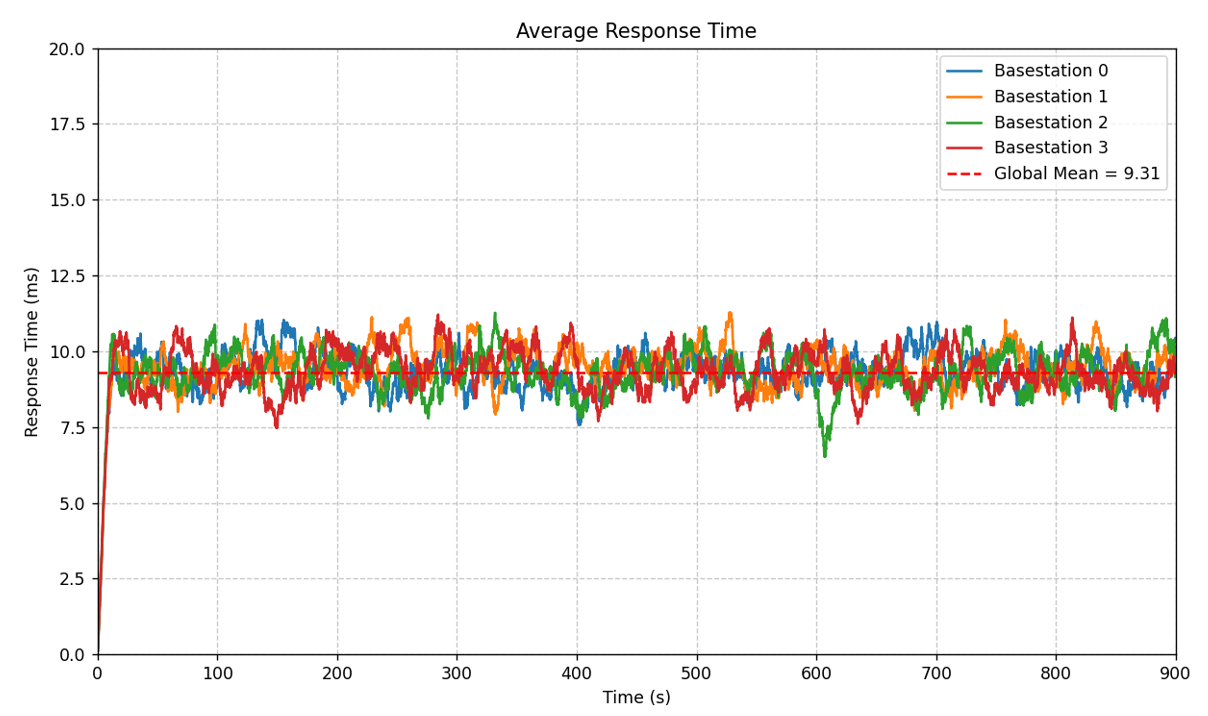
\includegraphics[width=0.8\textwidth]{rt_100.png}
        \caption{$N=100$}
    \end{subfigure}
    \caption{}
\end{figure}

\section{Increment of requests' load - ($\lambda=0.1,\ 1,\ 5$)}
In this case the mean response time remains comparable for the first two values of lambda, the third one shows a mean value of almost an order of magnitude of difference and a higher variability.

\begin{figure}[H]
    \begin{subfigure}{0.55\textwidth}
        \centering
        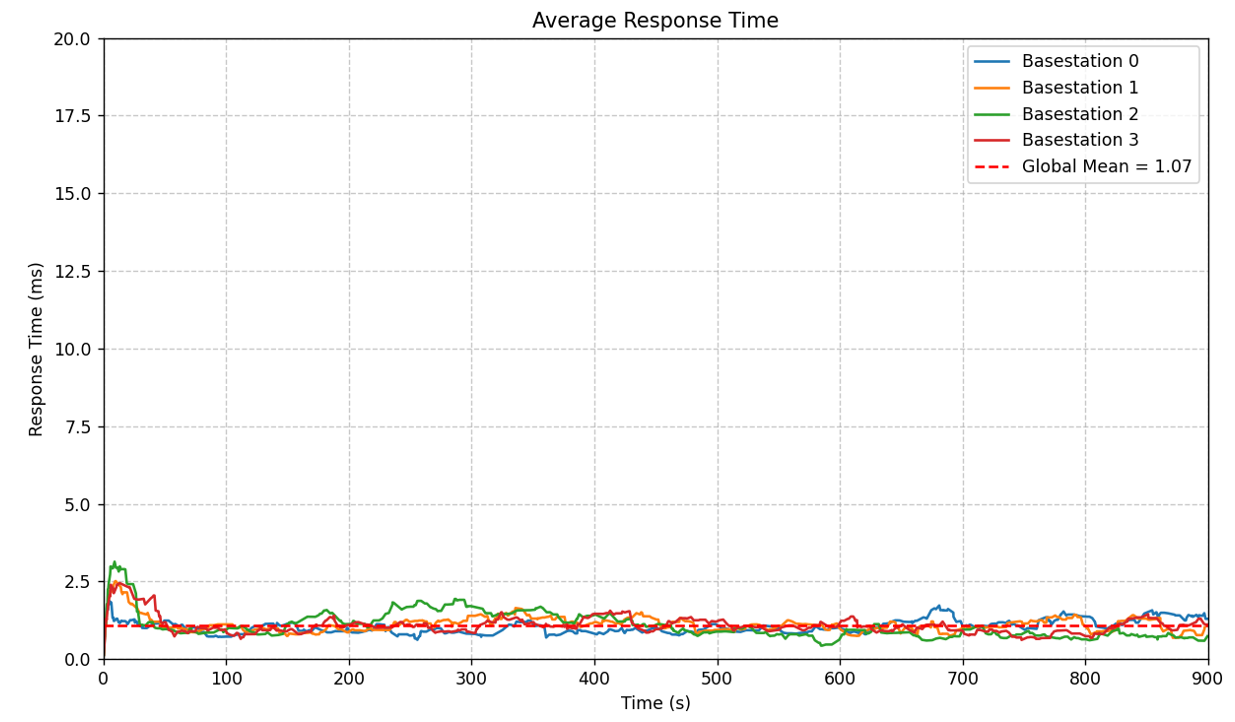
\includegraphics[width=0.8\textwidth]{rt_lambda_01.png}
        \caption{$\lambda = 0.1$}
    \end{subfigure}
    \begin{subfigure}{0.55\textwidth}
        \centering
        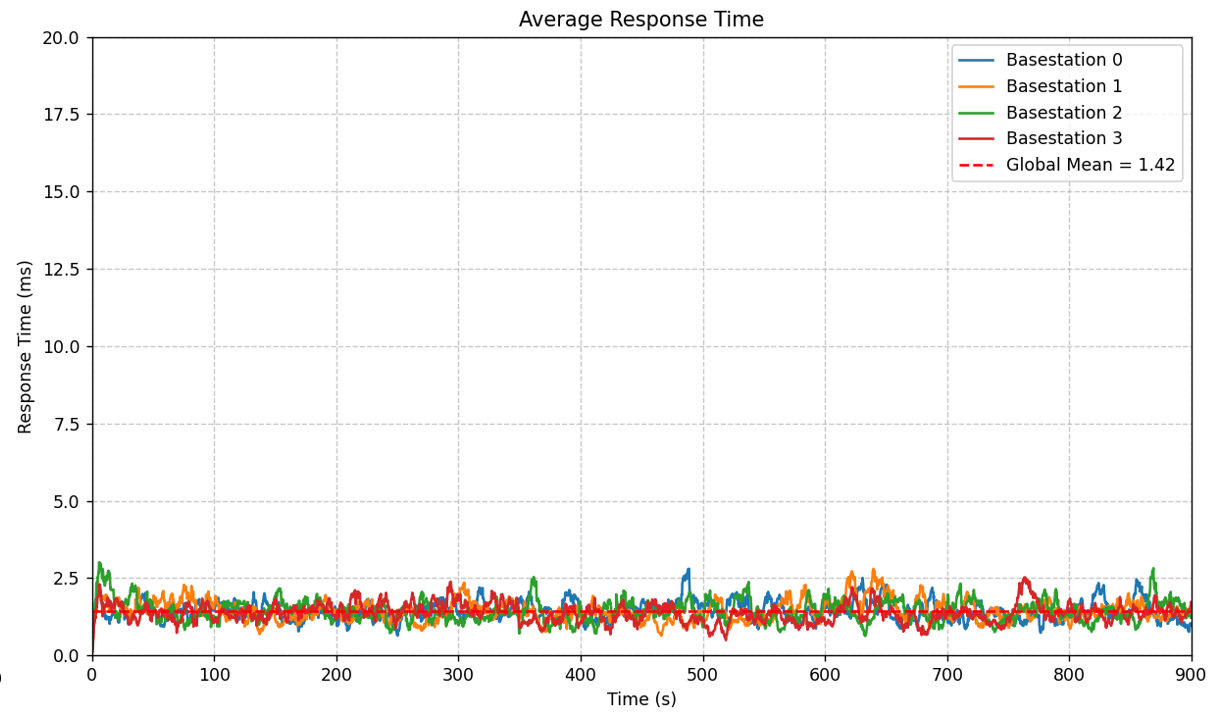
\includegraphics[width=0.8\textwidth]{rt_lambda_1.png}
        \caption{$\lambda = 1$}
        \label{rt_50}
    \end{subfigure}
    \begin{subfigure}{0.55\textwidth}
        \centering
        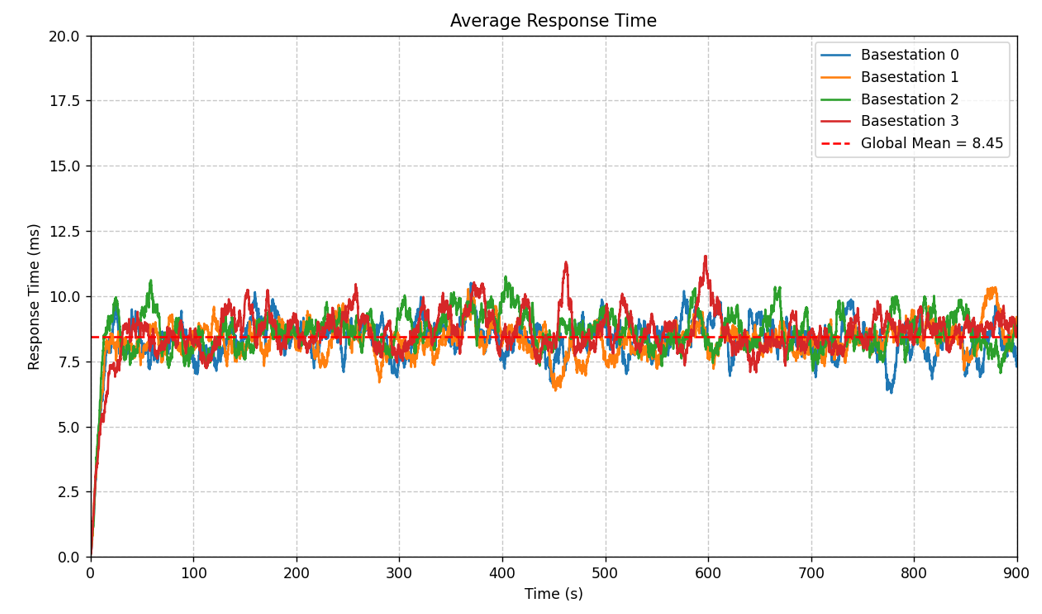
\includegraphics[width=0.8\textwidth]{rt_lambda_5.png}
        \caption{$\lambda = 5$}
    \end{subfigure}
    \caption{}
\end{figure}

\section{Monotonicity test}
This test evaluate if the output of the system follows a monotonic relation with any of the input parameters.

\subsection{Number of users}
This case has already been already analyzed in \autoref{nusers}.

\subsection{Service rate}
With the variation of the service rate ($\mu = 1000, \ 5000, \ 10000$) the mean response time changes drastically over the cases.

In particular in the first one there aer tho orders of magnitude of difference with the others.

\begin{figure}[H]
    \begin{subfigure}{0.55\textwidth}
        \centering
        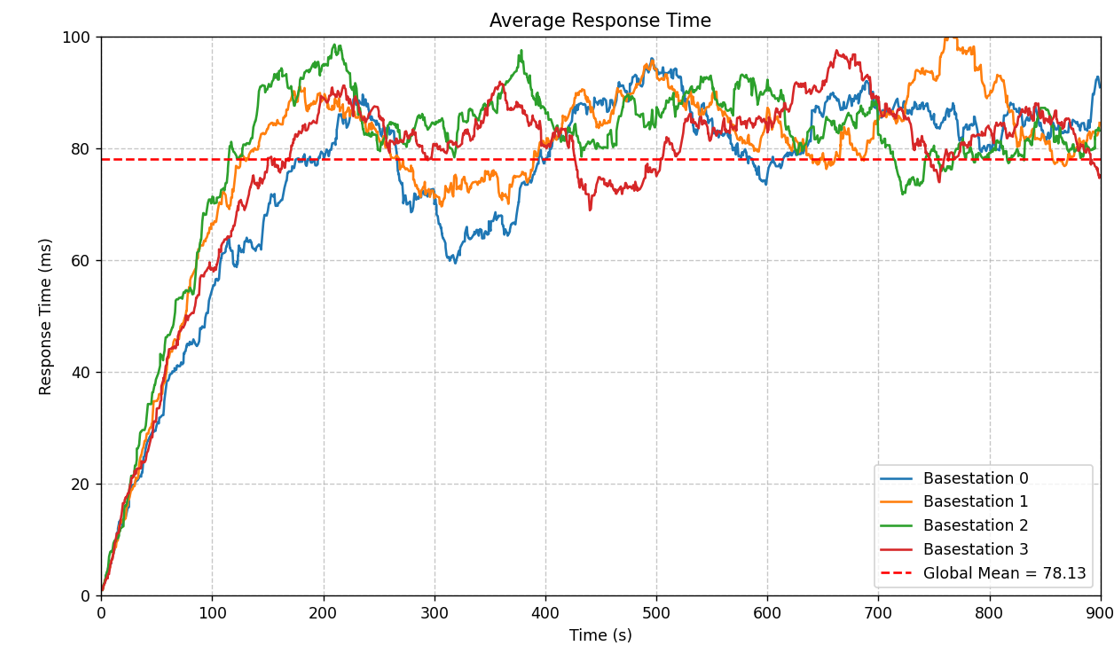
\includegraphics[width=0.8\textwidth]{rt_sr_1k.png}
        \caption{$\mu = 1000$}
    \end{subfigure}
    \begin{subfigure}{0.55\textwidth}
        \centering
        
\includegraphics[width=0.8\textwidth]{placeholder.jpg}
        \caption{$\mu = 5000$}
    \end{subfigure}
    \begin{subfigure}{0.55\textwidth}
        \centering
        
\includegraphics[width=0.8\textwidth]{placeholder.jpg}
        \caption{$\mu = 10000$}
    \end{subfigure}
    \caption{}
\end{figure}

\section{Verification against the theoretical model}
Now we compare the results of various simulations with those predicted by a theoretical model, which is described as follows.

\subsection{Theoretical analysis}
This is based mostly on \textit{queueing theory}, in particular on the $M|M|1$ model which describes our base stations, remembering the fact that they are characterized by a queue of finite length $k$.

Nowing that the service rate is equal to the product of the \textit{number of instructions processed per second} and the \textit{interarrival rate}
\[\mu = S\cdot \lambda\]

we compute the \textit{response time} for both configurations we simulated:

\textbf{Locally managed:}
\[t_r=\frac{1}{\mu-\lambda}\]

\textbf{Forwarding:}
\[t_r=D+\frac{1}{\mu-\lambda}\]

Where $D$ is a constant delay intrinsic in the system (i.e. network delay or computational delay)

In \autoref{th_a} and \autoref{th_b} we compare the results of theoretical and practical analysis in case of locally managed and forwarding.

\begin{figure}[H]
    \begin{subfigure}{0.55\textwidth}
        \centering
        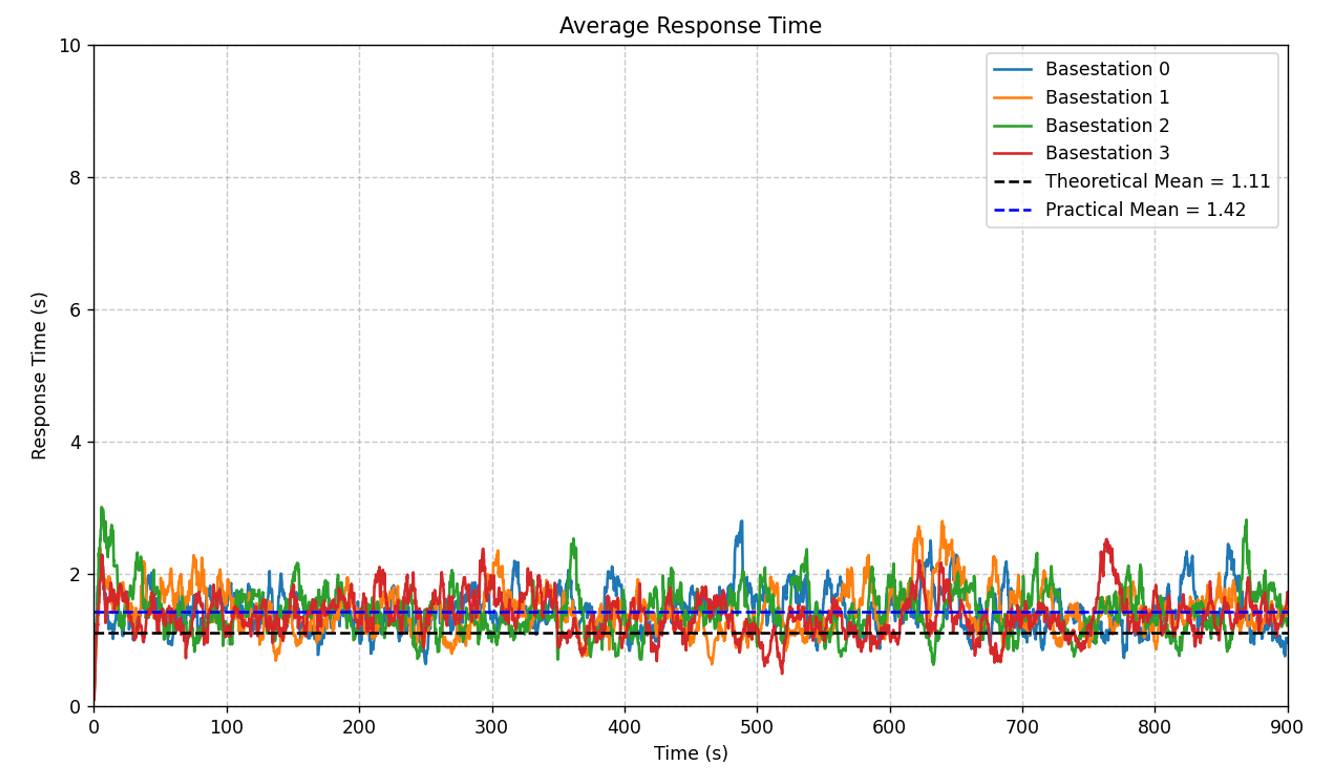
\includegraphics[width=0.8\textwidth]{th_rt_a.png}
        \caption{Case a.}
        \label{th_a}
    \end{subfigure}
    \begin{subfigure}{0.55\textwidth}
        \centering
        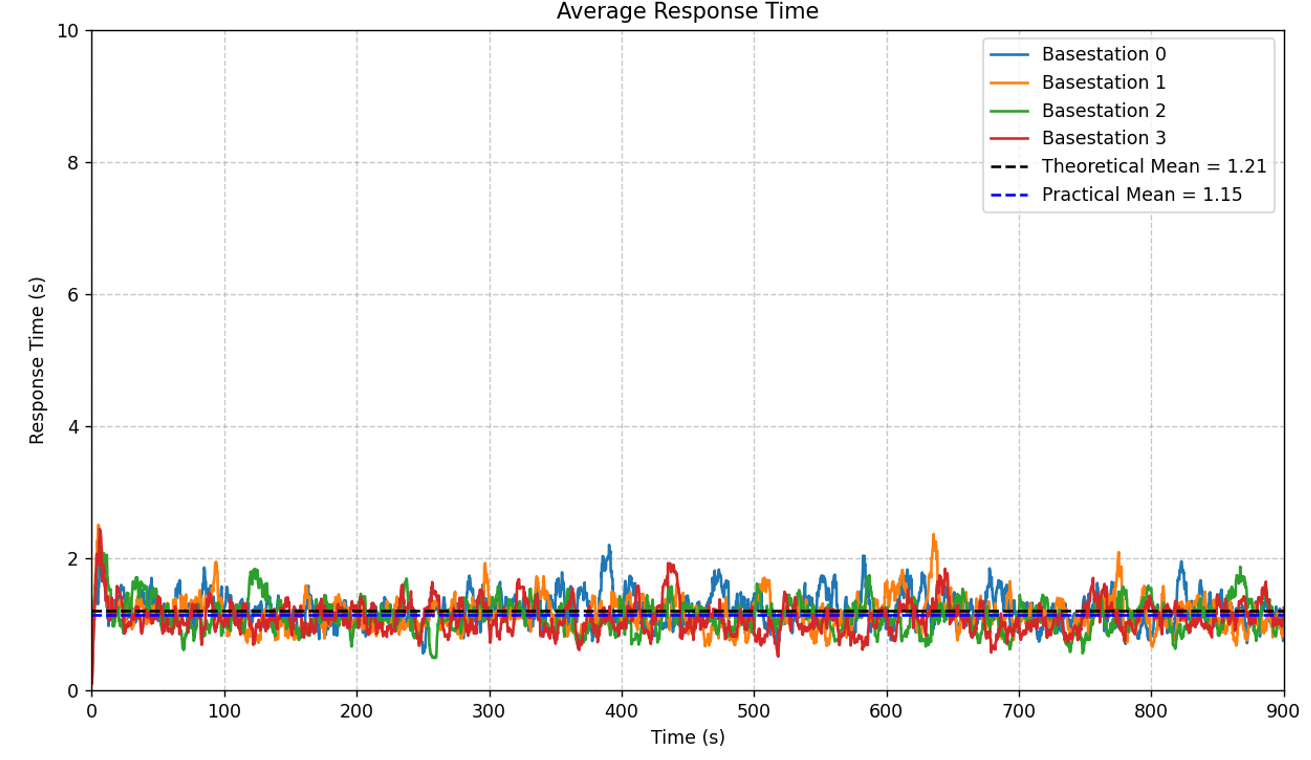
\includegraphics[width=0.8\textwidth]{th_rt_b.png}
        \caption{Case b.}
        \label{th_b}
    \end{subfigure}
    \caption{}
\end{figure}

\chapter{Calibration}
We now discuss how factors and other parameters have been chosen throughout the developement.

\section{Factors calibration}
The aim of this section is to fix the intervals of the factors to correctly reproduce reality in our system.

\subsection{Number of base stations}
This number depends on where is the area located geographically and on it's dimentions.
In suburban areas, are commonly spaced 2/3 km apart and in dense urban areas, they may be as close as 400/800 m apart\footnote{Source: \href{https://en.wikipedia.org/wiki/Cell_site}{Wikipedia}}.

\subsection{Number of users per base station}
This number changes in the range $[10, 50]$ depending on how much an area is effectively crowded.%\cite{prop_channel} -> questa roba mi fa incazzare dio mostro

\subsection{Warmup time analysis}

\appendix

\bibliographystyle{ieeetr}
\bibliography{bibliografia.bib}

\chapter{Simulation}
\chapter{Conclusion}
\end{document}